\chapter{Introduction}
\label{introduction}
\lhead{Chapitre 1 - Introduction}
\section{Contexte}

Chaque année à l'Université catholique de Louvain, et dans toute les autres universités, un étudiant est amené à devoir effectuer des choix au niveau du programme de cours qu'il va suivre. Même si ces choix demeurent plus restreint en bac qu'en master, le processus actuel représente une lourde tâche de travail pour le personnel en charge de la vérification de ces programmes et risque de s'amplifier encore plus avec le nouveau décret. 

En bachelier, cela se limite au choix d'une mineure de manière générale. La tâche est déjà plus compliquée lorsqu'il faut traiter le programme d'un étudiant qui recommence son année.

En master par contre, l'ensemble des choix est plus vaste. Le catalogue des programmes est plus versatile (Master 120, Master 60) et plus modulable. En effet, un étudiant doit choisir une ou plusieurs options. De plus, chacune d'entre elles est composée de cours obligatoires et optionnels. Ensuite, pour les programmes étalés sur deux ans, chacun des cours peut être suivi durant la première ou la deuxième année. Enfin, il faut prendre en compte les diverses équivalences lorsqu'un étudiant de notre faculté part en Erasmus, ou lorsqu'un étudiant étranger vient étudier dans notre université. Le processus de validation est donc plus complexe et nécessite considérablement plus de temps pour chacune des deux parties, à savoir la commission de programme du département d'informatique de l'École Polytechnique de Louvain - (\textbf{La commission INFO}) - et ses étudiants. 

En outre, la fédération Wallonie - Bruxelles (\textit{FWB}) a réalisé un décret qui a un impacte considérable sur comment, quand les étudiants  peuvent et doivent créer leur programme et choisir leur cours. Le but de cette réforme est de proposer des programmes plus à la carte,  afin que la structure des formations enseignées chez nous se calque sur celle des grandes universités anglo-saxonnes.

Cette réforme a pour conséquence de complexifier la gestion des programmes de master, mais surtout ceux de bachelier, offrant plus de liberté aux étudiants. Alors que le gros du travail se fait actuellement à l'aide d'un formulaire papier, il est urgent de passer à une version automatique pour simplifier la tâche au personnel et aux étudiants. 

\clearpage
\section{Problème}
Le problème est, une fois découpé, relativement simple à comprendre. Nous avons deux acteurs; \textit{la commission INFO} et les étudiants. 
La \textit{commission INFO} propose un catalogue de cours aux étudiants et plusieurs types de contraintes s'exercent sur chacun des cours de ce catalogue. L'étudiant doit se construire un programme de cours à partir du catalogue et \textit{la commission INFO} doit vérifier l'intégrité du programme de chaque étudiant. Il y a donc un processus de \textit{négociation} entre les deux parties, durant lequel \textit{la commission INFO} souligne les erreurs éventuelles pour être, par après,  corrigées par l'étudiant jusqu'à la validation de son programme.

Cependant, il faut garder à l'esprit que l'état du catalogue, des contraintes ou même des cours peut évoluer à tout moment. Comme mentionné plus haut, la \textit{FWB} peut émettre de nouvelles règles, de nouvelles lois dont l'impact peut bouleverser de façon relativement importante la structure et l'organisation des programmes. De plus, il est fréquent de voir certaines contraintes comme les crédits d'un cours, le semestre ou même le cycle durant lequel il est dispensé changer au cours des années.

L'encodage, l'interprétation, la connaissance et la vérification de l'ensemble de ces contraintes, qui ne sont parfois pas très explicites, sont à la charge de \textit{la commission INFO}.

L'image~\ref{fig:master_program} représente une vue de l'ensemble des cours, modules et contraintes du programme de \textbf{master} en informatique. Les nœuds représentent les différents cours, modules et programmes disponibles, tandis que les liens entre ces différents nœuds correspondent aux dépendances entres les cours. La complexité du graphe, malgré qu'il a été retravaillé et simplifié pour augmenter sa lisibilité, est assez évidente.

\begin{figure}
\centering
\caption{Programme de Master}
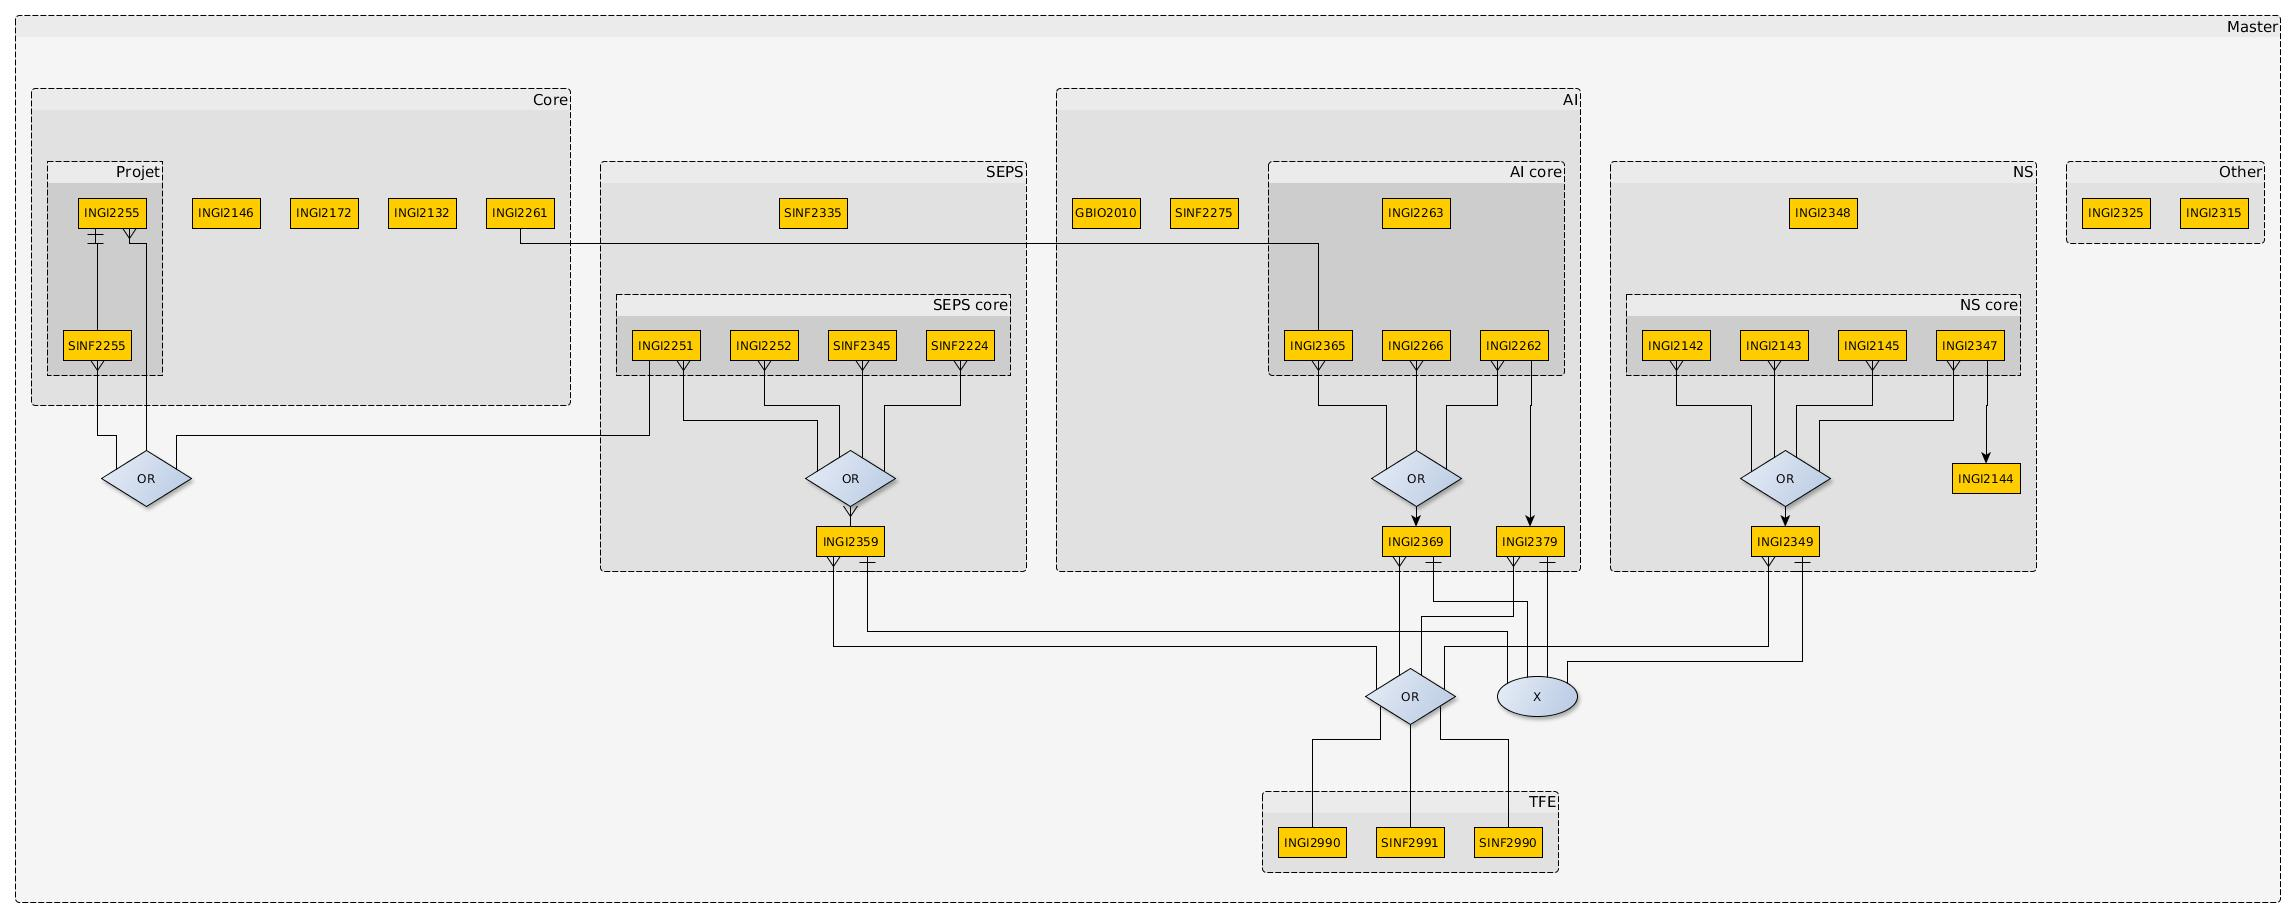
\includegraphics[angle=90, height=0.95\textheight, width=0.9\textwidth]{master_program}
\label{fig:master_program}
\end{figure}

Présentement, le processus de construction du programme de cours pour un étudiant est assez rudimentaire. Ce processus est représenté sur le diagramme ~\ref{fig:initial_process}

\begin{figure}
\centering
\caption{Processus actuel}
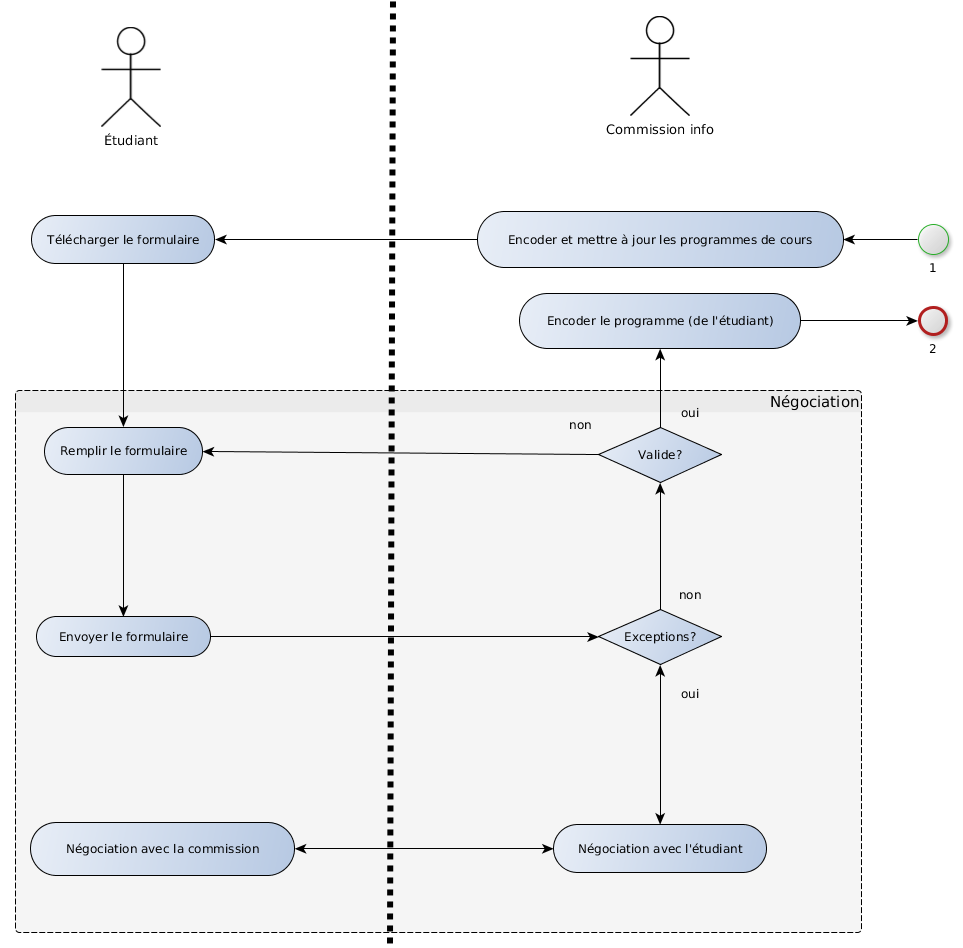
\includegraphics[width=\textwidth]{initial_process}
\label{fig:initial_process}
\end{figure} 

\textit{La commission INFO} commence par mettre à jour ses différents programmes de cours, puis crée le formulaire excel contenant le programme de cours et enfin le mets en ligne sur le portail de la faculté (afin qu'il soit téléchargeable par les étudiants par après).

L'étudiant télécharge le formulaire contenant le programme de cours et le remplit. 

Ici commence la phase de négociation entre \textit{la commission INFO} et les étudiants. Les deux parties vont s'échanger un formulaire que l'étudiant va compléter et \textit{la commission INFO} vérifier. L'échange va se poursuivre jusqu'à ce que le programme soit valide. 

L'étudiant complète d'abord son formulaire en tenant compte des spécifications du programme. S'il est en bac par exemple, il y a des cours obligatoire à prendre chaque année. S'il est en master, il y a une option à choisir, des cours obligatoires, etc. Il peut cependant exister des exceptions dans les différents programmes qui permettent d'enfreindre ces spécifications. Par exemple, un étudiant en provenance d'une autre université ou d'une autre faculté peut avoir déjà suivit l'équivalent d'un cours obligatoire dans son université ou sa faculté d'origine. Il va devoir rendre un formulaire qui ne respecte pas les contraintes initiales, justifier ces exceptions et négocier leur acceptation avec \textit{la commission INFO}.

Il envoie son formulaire par mail à \textit{la commission INFO}.

\textit{La commission INFO} réceptionne le formulaire. Elle vérifie la validité du programme. Si l'étudiant revendique des exceptions dans son programme, elle vérifie si elle sont fondées ou non. Si le programme ou ces exceptions ne sont pas validées, la \textit{commission INFO} peut demander d'amples informations à l'étudiant ou négocier avec lui et, si nécessaire, il est demandé à l'étudiant de compléter sont formulaire avec les informations qu'il manque. Le processus de validation recommence ainsi à zéro. Si le programme est valide, il est encodé. 

Le processus actuel, que ce soit en bac ou en master, se déroule essentiellement à l'aide d'une feuille de papier et les négociations par mail ou oralement. L'étudiant recherche les informations dont il a besoin sur le site de l'UCL, auprès de ses collègues ou encore sur les forums de cours, complète le formulaire et le dépose au secrétariat.

\textit{La commission INFO} quant à elle, effectue une vérification à la main de ces formulaires, négocie oralement ou par mail avec les étudiants si besoin est. 
Informatiser ce processus à l'air du web 3.0 est une nécessite plus qu'absolue.



\section{Motivation}
Reprenons le diagramme \ref{fig:initial_process} représentant le processus de création de programme tel qu'il se déroule actuellement. 

Le mot d'ordre est \textbf{automatisation}.

Comme présenté dans la section précédente, certaines étapes sont sources de beaucoup de problèmes pour \textit{la commission INFO}.

\begin{description}
  \item[Encodage/Mise à jour des programmes de cours] Cette étape se fait manuellement. De plus, la \textit{ commission INFO} doit, une fois le programme encodé, compléter à la main le formulaire excel qui va être utilisé par les étudiants. 
  \item[Vérification des programmes des étudiants]  Cette étape se fait manuellement. 
  \item[Négociation avec les étudiants] Cette étape se fait oralement ou par mails.
\end{description} 

Avant toute chose, il y a beaucoup d'informations qui sont échangées entre les deux parties, que ce soit implicitement ou explicitement.

Les données implicites correspondent aux informations relatives aux étudiants, comme l'historique de leur parcours universitaire, qui pourrait par exemple justifier certaines des exceptions mentionnées précédemment. Ces données ne concernent pas directement les choix faits par les étudiants au niveau de leur programme de cours, mais sont plutôt des méta-informations qui complètent leur profile. 

Les données explicites correspondent aux choix faits par les étudiants. Ces données concernent les
\begin{itemize}
\item les choix faits par les étudiants au niveau de leur programmes de cours;
\item les justifications des étudiants à propos des exceptions de leur programme par rapports aux règles et structures fixées par le programme de cours suivit. 
\end{itemize}

Il faut aussi garder une trace de ce que l'étudiant a suivi et réussi les années précédentes. En effet, il est nécessaire de savoir quel cours un étudiant à réussi l'année précédente pour attribuer les différentes dispenses lorsqu'il recommence son année par exemple.

Dès lors, la \textit{commission INFO} doit pouvoir valider le programme d'un étudiant lorsque celui-ci l'a réussi. 

Il est donc indispensable d'inclure dans la solution une base de données pour y stocker toutes ces informations, afin qu'elles soient à disposition des deux parties à tout moment.

Différents points du processus actuel \ref{fig:initial_process} doivent être automatisés.

Le premier point identifié se situe au niveau du support utilisé par l'étudiant et \textit{la commission INFO}, le formulaire excel, pour ajouter de l'information sur le programme de cours. Tout d'abord, \textit{la commission INFO} doit générer manuellement ce formulaire, en y incluant les cours et différentes options du programme de cours en question. Ajouter les différents blocs, cours et leur crédits respectifs est assez contraignant sur un simple tableur. De plus, beaucoup d'erreurs peuvent êtes laissées par l'étudiant lorsqu'il complète celui-ci. Certes, il y a certains moyen à disposition sous Excel (en utilisant des macros), pour vérifier certaines contraintes du programmes (comme le nombre de crédits d'un module par exemple) mais ceux-ci peuvent être ignorés par l'étudiant, et doivent de toute façon être revérifiées par après par \textit{la commission INFO}. 

\textbf{Le premier point} de la solution proposée est donc d’offrir une plate-forme permettant aux acteurs d'échanger ces différentes informations.

Deuxièmement, l'étape de complétion du formulaire par l'étudiant doit être améliorée. Il n'est pas possible de mettre des informations concernant les contraintes autre que numéraires dans le formulaire excel utilisé pour le moment. La plate-forme doit donc inclure des vues représentant de façon claires et concises les différentes contraintes des programmes de cours. De plus, ces contraintes doivent être aisément en-codables, gérables et modifiables. 

Troisièmement, l'étape de vérification des contraintes, pour valider un programme d'étudiant est coûteuse en temps pour \textit{la commission INFO}, alors que cela ne prendrait que quelques secondes pour un ordinateur. Un module pour vérifier ces contraintes doit être inclus dans la plate-forme

Quatrièmement, il faut s'attaquer au processus de négociation qui amène l'étudiant, en relation avec \textit{la commission INFO}, à construire un programme valide. Tant que le programme de l'étudiant n'est pas valide, l'étudiant doit corriger son programme en tenant compte du feedback de \textit{la commission INFO}. La \textit{commission INFO} doit contacter l'étudiant en pointant les parties non correctes de son programme et l'étudiant doit à son tour comprendre les requêtes de \textit{la commission INFO}, puis tenter de les résoudre ou de les corriger. Par mail ou par papier, cela peut être très long. 
\clearpage


\section{Objectifs}
De manière générale, le but de cette application est d'automatiser la gestion des programmes de cours. 


Le \textit{pré-objectif} est d'être indépendant de la base de données EPC. Pour des raisons institutionnelles, l'équipe EPC est surchargée en plus d'être réticente à donner un accès au données. Dans le futur, peut être l'outil pourrait échanger des données avec EPC ou même être intégré, mais ce ne sera pas pour immédiatement. C'est pourquoi il faut pouvoir importer les données de façon efficace et intuitive.
 
La solution doit être maintenable et évolutive. En effet, la structure des programmes est en constante évolution. De plus, il est probable que la commission de programme découvre de nouveaux besoins qui devront être implémentés à l'avenir. Il est donc primordial de structurer l'application intelligemment pour que celle-ci soit modulaire et qu'on ne doive pas repartir de zéro lors de développement ultérieurs.

La \textit{commission INFO} doit pouvoir apporter des catalogues de cours sur l'application. Un catalogue de cours est un ensemble de programmes de cours, contenant les différents modules, cours et dépendances. Un programme de cours est un cursus qu'il est possible de suivre dans la faculté, comme par exemple le programme de MASTER destinés aux SINFs (SINF2M), le programme de passerelle (SINF1PM) ou encore celui de BAC destinés aux ingénieurs civils (FSA1BA).  

Les informations des programmes de cours  doivent pouvoir être téléchargées depuis l'application ainsi qu'être mises à jour. En effet, les programmes de cours sont sujets régulièrement à des changements. Il est donc nécessaire que ces données ne soient pas ajoutées en \textit{"en dur"} dans l'application. De plus, ces données doivent être visibles de manière synthétique par la commission (vue \textit{admin}).

Il doit y avoir un historique des différentes versions des programmes de cours mis en ligne par la \textit{commission INFO} tout aux long des années académiques,pour gérer l'évolution de ceux-ci et pouvoir permettre aux étudiants (à qui cela est permis) de choisir dans leurs programmes des cours d'anciens catalogues, en cas de report de note par exemple.
 
Les étudiants doivent pouvoir construire leur programmes, en choisissant les cours et les modules qu'ils vont suivre chaque année. L'application doit leur dire si leur programme est cohérent ou non.

Au niveau de ces contraintes, il doit y avoir une certaine souplesse. Il n'est pas possible d'avoir une vision \textit{manichéenne} à ce niveau.

Il doit être possible aux étudiants d'attirer l'attention sur certaines parties de leur programme en y ajoutant un commentaire pour poser une question, ou pour justifier un choix.

En tant qu'étudiant il doit être possible de
\begin{itemize}
\item se créer un compte utilisateur avec son adresse mail UCL:
\item sélectionner la version du catalogue de cours avec laquelle il va travailler;
\item se créer un programme en choisissant un des programmes de cours disponibles à suivre;
\item choisir les différents modules de cours à suivre, option, tronc commun, \ldots ;
\item avoir une vue sur les différentes années du programme qu'il suit (les deux années de MASTER par exemple);
\item configurer son programme par année académique, en choisissant les cours que l'on va suivre durant les différents semestres;
\item voir les contraintes qui ne sont pas respectées, par exemple, le nombre de crédits manquants pour valider un module, ou encore les dépendances d'un cours;
\item pouvoir soumettre à la validation son programme, même s'il ne respecte pas toutes les contraintes;
\item pouvoir communiquer avec la commission info à travers l'application; par exemple justifier une contrainte non respectée par écrit. ("J'ai déjà suivit un cours très semblable durant mon cursus dans la faculté X à l'université Y").  
\end{itemize}

La \textit{commission INFO} doit pouvoir:
\begin{itemize}
\item vérifier, de la façon la plus automatisée possible, le programme d'un étudiant;
\item importer les différents programmes de cours dans l'application;
\item mettre à jour les données relatives à ces programmes;
\item être notifié lorsqu'un étudiant envoie son programme à la validation;
\item accéder aux programmes des étudiants;
\item communiquer avec les étudiants à travers l'application;
\item marquer les années précédentes des étudiants comme réussies ou ratées.
\end{itemize}

Le processus auquel nous désirons arriver est illustré sur l'image \ref{fig:desired_process};

\begin{figure}
\centering
\caption{Processus désiré}
\label{fig:desired_process}
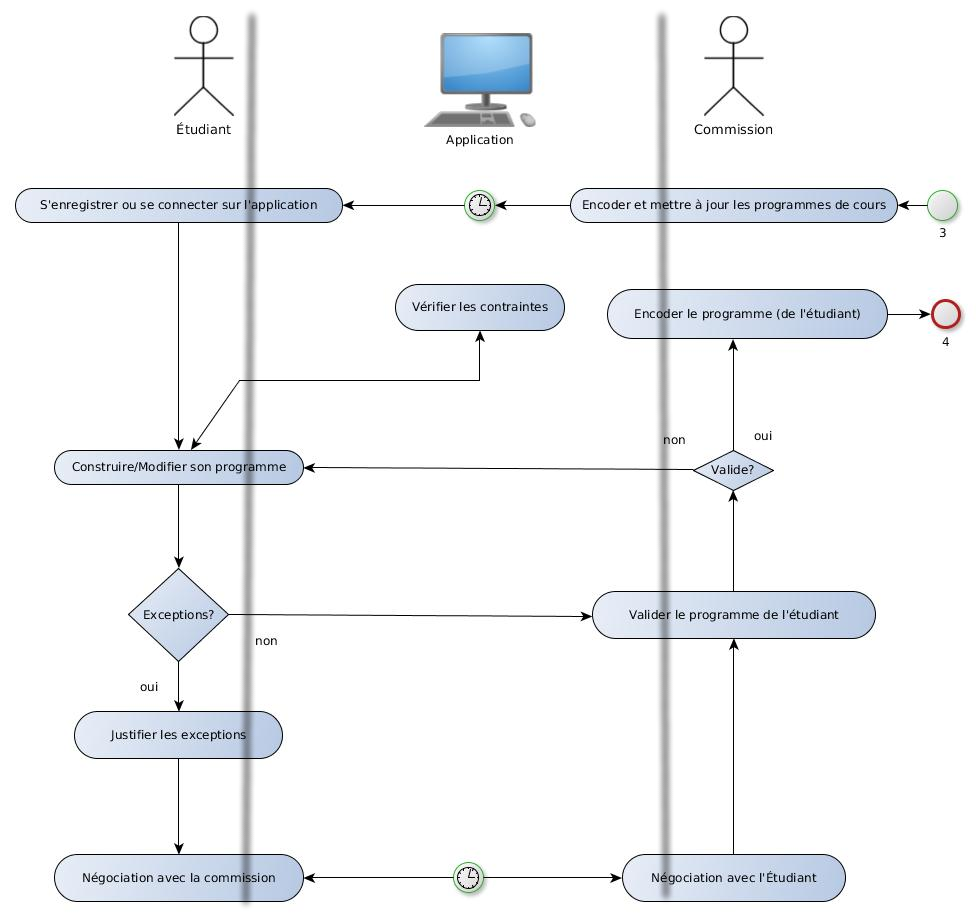
\includegraphics[width=\textwidth]{desired_process}
\end{figure}


La \textit{commission de programme} importe et mets à jour les différents programmes à l'aide d'un fichier yEd ou Excel externe qui est ensuite importé dans l'application

L'étudiant se connecte à l'application, crée son programme de cours, et le configure pas à pas en réduisant au maximum le nombre de contraintes non vérifiées. Pour les contraintes non vérifiées restantes, il insère en commentaire les justifications à ces exceptions. 

L'étudiant envoie son programme à la validation. 

\textbf{Négociation} - La \textit{commission de programme} récupère la requête de validation. L'application lui montre les contraintes qui ne sont pas respectée. La \textit{commission de programme} regarde ensuite les justifications de l'étudiant. Si elle ne sont pas suffisante, la \textit{commission INFO} refuse la demande de validation et commente sa validation en expliquant pourquoi certaines justifications ne sont pas suffisantes. 

Le processus de négociation se répète jusqu'à ce que le programme de l'étudiant soit valide. S'il n'y a pas d'exceptions, l'application peut immédiatement vérifier si le programme de l'étudiant est valide et le valider (si c'est le cas) ou demander de modifier son programme (si il n'est pas valide).





